\lvli{Introduction}

In this experiment we analyzed the behavior of an FBG (Fiber Bragg Grating). The FBG uses the Bragg Mirror, which is a specific type of photonic crystal that acts as a mirror for a given range of frequencies. This photonic crystall can be modeled as a multilayer film where two materials with different refractive index are alternated.Imagining an ideal Bragg mirror the reflected wavelength is defined as $\lambda_{BRAGG} = \frac{2\pi}{k_{BRAGG}}$ where $k_{BRAGG}$ it is the propagation constant of the phase and respects this rule $k_{BRAGG} \cdot (L_1 + L_2) = m \cdot \pi$ with $m \in \mathbb{N}$ and $L_1, L_2$ are the two lengths of the films. By inserting a Bragg mirror into the fiber we obtain a mechanical coupling between the two in particular in compression and elongation, in fact pulling the fiber is also pulled the mirror and then modified the period $(L_1 + L_2)$ which in turn changes $\lambda_{BRAGG}$. From this physical effect we can then relate elongation with the reflected frequency. This mirror, however, is also sensitive to temperature variations, in fact, in addition to creating an expansion or compression of the period, it introduces a variation of the silica refraction index induced by the thermo-optic effect.

The setup we use is composed of an optical amplifier that produces broadband light that is inserted into a fiber containing an FBG, the light that is reflected then passes through an optical circulator that sends it to a spectrum analyzer (Fig.\ref{fig:setup}).
\begin{figure}[h]
    \centering
    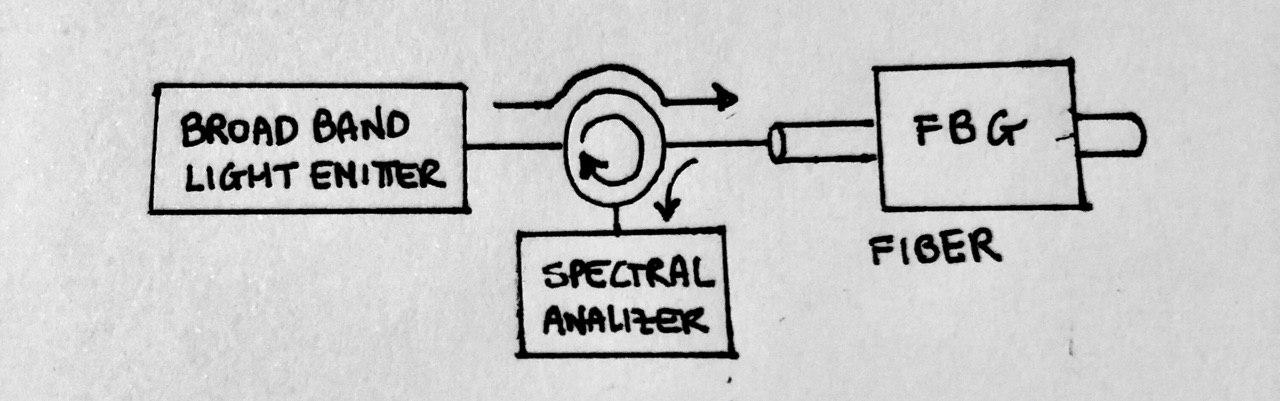
\includegraphics[scale=0.3]{img/setup.jpg}
    \caption{Setup.}
    \label{fig:setup}
\end{figure}

What is done in this experiment is to measure the reflected wave frequency according to the applied elongation. In this case the elongation is performed by turning a circular manual tensor (ring): each rotation corresponds to an elongation of $0.5 [mm]$ and on the ring there are 50 notches and therefore we have an elongation of $0.01 [mm] $for notch. Our fiber started from a length of $14 [mm]$ and we elongated it by $1.5 [mm]$. The measurements we have performed are shown in (Tab.\ref{table:measures}), where for each rotation the value of the reflected frequency calculated by eye was reported. The table has three measuring columns because more consecutive measurements have been made starting from $14 [mm]$ and reaching $14.75 [mm]$ then going back to $14 [mm]$ and then returning to $14.7 [mm] $. The table also specifies with $x$ the measurements where the spectrum was stored for computer analysis.
\begin{table}[h]
  \centering
  \begin{tabular}{c|c|c|c}
      Position [mm]  &  $\lambda_B$  [nm]  &  $\lambda_B$  [nm]  &  $\lambda_B$  [nm]  \\
      \hline
      14     &  1534,691     &  1534,682(x)  &  1534,682     \\
      14.05  &  1534.861     &  1534.87      &  1534.861     \\
      14.1   &  1535.032     &  1535.032     &  1535.041(x)  \\
      14.15  &  1535.229     &  1535.186     &  1535.212     \\
      14.2   &  1535.391     &  1535.357     &  1535.391(x)  \\
      14.25  &  1535.604(x)  &  1535.562(x)  &  1535.587     \\
      14.3   &  1535.784     &  1535.749     &  1535.767(x)  \\
      14.35  &  1535.937     &  1535.92      &  1535.946     \\
      14.4   &  1536.125     &  1536.108     &  1536.108(x)  \\
      14.45  &  1536.305     &  1536.262     &  1536.305     \\
      14.5   &  1536.509(x)  &  1536.45 (x)  &  1536.467(x)  \\
      14.55  &  1536.663     &  1536.646     &  1536.646     \\
      14.6   &  1536.851     &  1536.851     &  1536.842(x)  \\
      14.65  &  1537.03      &  1537.005     &  1537.005     \\
      14.7   &  1537.184     &  1537.184     &  1537.184(x)  \\
      14.75  &  1537.389(x)  &  1537.389     &  1537.38      \\

  \end{tabular}
  \caption{Measures.}
  \label{table:measures}
\end{table}
From a first analysis we obtain the curve shown in (Fig.\ref{fig:firstAnalisy}).
\begin{figure}[h]
    \centering
    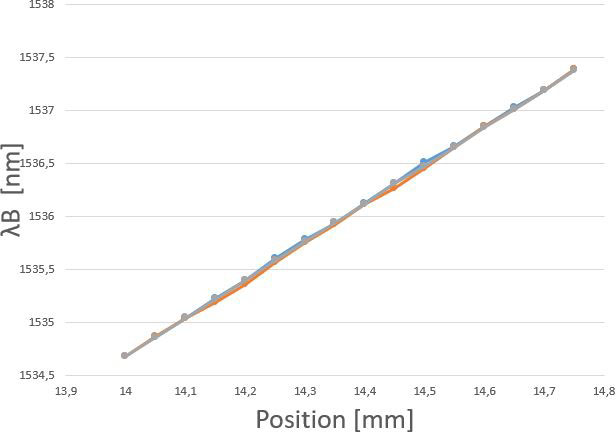
\includegraphics[scale=0.7]{img/firstAnalisy.jpg}
    \caption{First analisy.}
    \label{fig:firstAnalisy}
\end{figure}


\newpage
\lvli{Analysis}
First of all, the 13 files were imported. They contain the data related to the spectra measured by the spectrometer and contain: the two values of starting frequency and frequency step in THz; and then the list of reflected power values read in dB. The importation was made by converting the frequency values into wavelength values through the physical relation $\lambda = \frac{c_0}{f}$, to each of these values the corresponding power value has been assigned as shown in (Fig.\ref{fig:spectralPower}). From this figure it is also possible to clearly identify the peak to be analyzed, since while the signal has values lower than $-50[dB]$ and it has a value of approximately $-30[dB]$.
\begin{figure}[h]
    \centering
    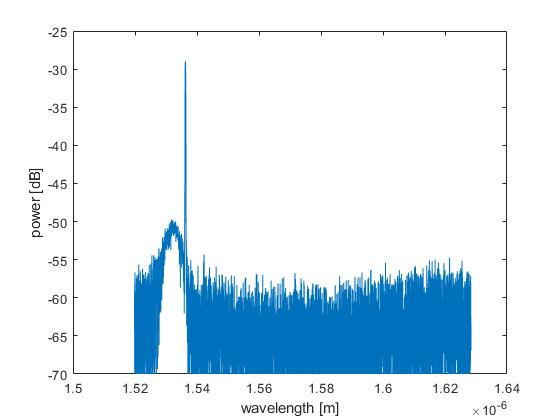
\includegraphics[scale=0.7]{img/spectralPower.jpg}
    \caption{Spectral power for 14[mm] of elongation.}
    \label{fig:spectralPower}
\end{figure}
A questo punto per ogni file viene cercato il valore della lunghezza d'onda corrispondemte al punto di massimo; per migliorare l'analisi viene eseguita un'interpolazione dei punti attraverso una funzione quadratica. Un punto chiave è stato scegliere quali punti considerare nell'approssimazione. Il primo tentativo è stato mediante un'approccio classico, si è scelto di considerare tutti i punti che sono sopra il 90\% del picco che ha comportato una soluzione come in (Fig.\ref{fig:quadratic_fit_scale}), da come si può vedere in questa immagine ci sono un po' di punti intorno al picco che aggiungono del rumore, la scelta successiva sarebbe stata quindi optare per una percentuale maggiore ma così facendo si sarebbe dovuto calcolare a mano per ogni spettro il valore di percentuale ottimale; invece si è scelto un'altro approccio. La soluzione alternativa è stata basata sulla caratteristica di simmetria del picco e segue il seguente approccio: partendo dal punto massimo ci si sposta lateralemente fino a quando non si trovano punti con valori decrescenti, l'esempio di filtraggio dei punti è mostrato in (Fig.\ref{fig:quadratic_fit}).

\begin{figure}[!htb]
  \minipage{0.32\textwidth}
    \centering
    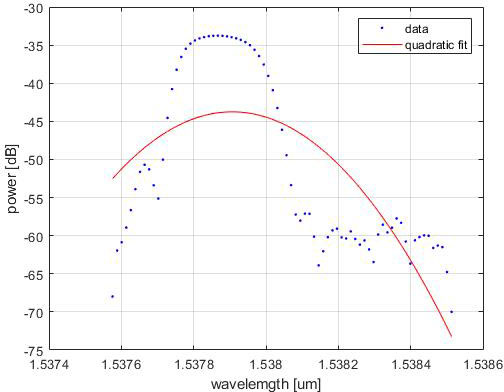
\includegraphics[scale=0.4]{img/quadratic_fit_scale_90.jpg}
    \caption{Quadratic fit scale 90\%.}
    \label{fig:quadratic_fit_scale}
  \endminipage\hfill
  \minipage{0.32\textwidth}
    \centering
    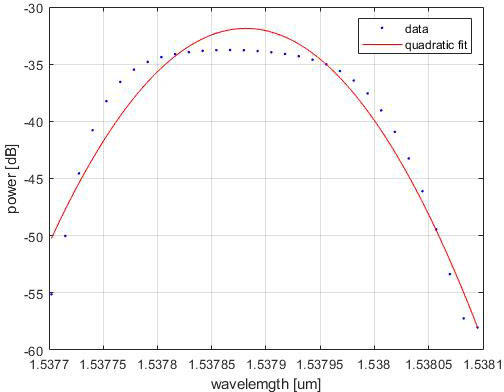
\includegraphics[scale=0.4]{img/quadratic_fit.jpg}
    \caption{Quadratic fit descending cutting mode.}
    \label{fig:quadratic_fit}
  \endminipage
\end{figure}

A questo punto si è messo in relazione i valori delle lunghezze d'onda appena calcolate con in valori di elongazione come mostato in (Fig.\ref{fig:spins}), avendo impostato i $14[mm]$ come nostro valore di 0 otteniamo un'elongazione di $0.75[mm]$. Da qui abbiamo proceduto con un fit lineare per poter ricavare il coefficiente angolare che corrisponde a $a = \frac{\Delta \lambda}{\mu \epsilon} = 3.588 \cdot 10^{-3}$, esso contiene l'informazione della deformazione del FBG che dipende dalla temperatura e dall'elongazione.
\begin{figure}[h]
    \centering
    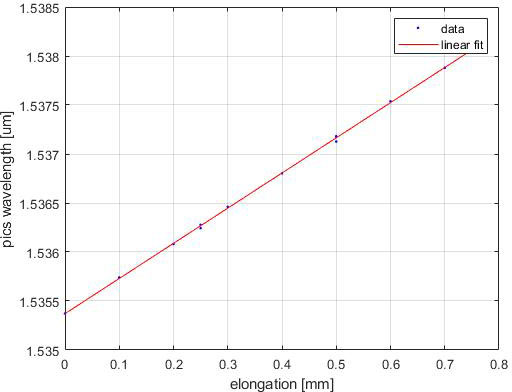
\includegraphics[scale=0.7]{img/spins.jpg}
    \caption{Elongation.}
    \label{fig:spins}
\end{figure}
 Supponendo che la temperatura all'interno della stanza fosse omogenea e che abbiamo svolto l'esperimento in un tempo sufficientemente breve l'effetto della temperatura diventa trascurabile rispetto a quello dell'elongazione. Questo viene anche confermato dall'andamento lineare dei dati ottenuti che si distacca dalla retta di fit di soli $RMSE = 1.6 \cdot 10^{-5}$. Da questo valore possiamo calcolare la sensibility dello strumento mediante la formula:
$$s = \frac{L}{a} = 0.0865[\mu \epsilon]$$
con $L=310.5[mm]$ la lunghezza della fibra a riposo.


\newpage
\lvli{Conclusion}
Il valore ottenuto è molto simile ai valore tipico per sensori di questo tipo:
$$\Delta(\mu\epsilon) = \frac{1 [pm]}{ 1.2 [\frac{pm}{\mu\epsilon}]} \approx 0.8 [\mu \epsilon]$$
L'andamento dei dati raccolti è stato ottimo perché hanno prodotto un andamento lineare come ci aspettavamo con un discostametno di $RMSE = 1.6 \cdot 10^{-5}$. Avendo eseguito le misure sia in contrazione che in elongazione abbiamo avuto la possibilità di controllare l'esistenza o meno di un comportamento di isteresi. I dati raccolti sebbene molto pochi suggeriscono la mancanza di isteresi visto il valore basso di RMSE.

%% DOMANDE PROF
% 1) ho un fattore 10 che non mi torna
% 2) c'è qualche modo in cui possa ricavarmi l'incertezza sulla sensibility?
% 3) c'è altro che si può aggiungere?
% 4) lo spettometro legge potenza? in dB?
